\section{Deep Learning Foundations}
\label{sec:dl_theory}
The automation of radargram analysis requires models capable of learning  representations from high-dimensional data.
Deep Learning (DL) provides a family of techniques that build such representations by stacking multiple layers of non-linear transformations, enabling the extraction of progressively more abstract features from raw inputs.
In this thesis we focus on a specific subset of DL models for image processing, namely Convolutional Neural Networks (CNNs) and Generative Adversarial Networks (GANs), which form the backbone of the proposed Sim-to-Real translation and anomaly detection pipeline.

\subsection{Convolutional Neural Networks (CNNs)}
CNNs are the backbone of modern computer vision.
Unlike fully connected networks, CNNs employ \textbf{convolution operations} that are translation equivariant, meaning that if a pattern is detected at position $(i,j)$ in the input, the same feature map will appear at a shifted position $(i+\Delta i,j+\Delta j)$ in the output, enabling consistent detection regardless of spatial location.
A discrete 2D convolution between an input $I$ and a kernel $K$ is defined as:
\begin{equation}
(I * K)(i, j) = \sum_m \sum_n I(i+m, j+n)\, K(m, n)
\end{equation}
This allows the network to detect local patterns (edges, textures) regardless of their position in the image.
Through pooling layers and strided convolutions, CNNs build an expanding \textbf{receptive field}, allowing deeper layers to capture broader spatial dependencies.

\begin{figure}[t]
    \centering
    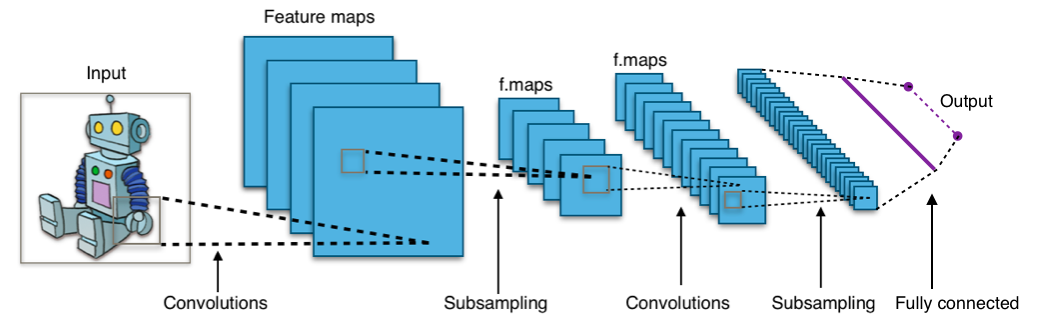
\includegraphics[width=0.9\linewidth]{images/typical_cnn}
    \caption{Typical architecture of a Convolutional Neural Network (CNN). Early layers (left) extract local features such as edges and textures via small convolutional kernels, while deeper layers progressively aggregate these into more global representations of shapes and contextual patterns (right). Adapted from~\cite{wikimedia_typical_cnn}.
    \label{fig:typical_cnn}}
\end{figure}

From a functional perspective, CNNs exploit local connectivity and weight sharing, whereby the same kernel parameters are applied across all spatial locations to efficiently model spatially localized patterns such as edges, textures, and small-scale structures that are ubiquitous in radargrams.
The depth of the network controls the size of the effective receptive field and thus the range of spatial dependencies that can be captured: early layers capture local features and fine-scale patterns (e.g., speckle, small hyperbolas), while deeper layers integrate these into more global representations of shapes and broader contextual patterns (e.g., extended stratigraphic horizons, large-scale clutter distributions).
These properties make CNN-based architectures naturally suited for both deterministic tasks (e.g., denoising, segmentation) and generative modelling of RS data.

\subsection{Encoder–Decoder Architectures (U-Net)}
For tasks like image-to-image translation and semantic segmentation, preserving spatial information is vital. The U-Net architecture~\cite{Ronneberger_2015} introduces a symmetric encoder–decoder structure:
\begin{itemize}
    \item \textbf{Contracting Path (Encoder):} Captures context and reduces spatial resolution through successive convolution and downsampling operations, progressively increasing the number of feature channels.
    \item \textbf{Expanding Path (Decoder):} Restores spatial resolution for precise localization, typically using transposed convolutions or upsampling followed by convolutions, progressively reducing the number of feature channels.
    \item \textbf{Skip Connections:} Direct links between encoder and decoder layers of the same resolution. These are critical for gradient flow and for recovering fine-grained spatial details lost during downsampling, by concatenating high-resolution feature maps from the encoder with the upsampled features in the decoder.
\end{itemize}

\begin{figure}[t]
    \centering
    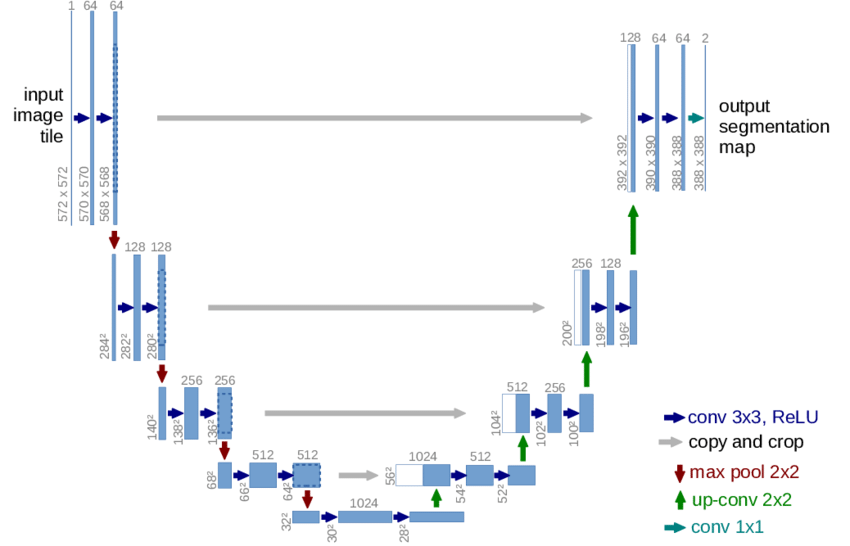
\includegraphics[width=\linewidth]{images/unet_original}
    \caption{Canonical U-Net architecture with a contracting encoder path (left) and a symmetric expanding decoder path (right), connected by skip connections that fuse high-resolution and low-resolution features. Adapted from Figure~1 in~\cite{Ronneberger_2015}.}
    \label{fig:unet_architecture}
\end{figure}

Originally proposed for biomedical image segmentation, U-Net was designed to produce pixel-wise classification maps, effectively performing semantic segmentation by assigning a class label to each pixel.
The combination of a deep encoder (to capture global context) with skip connections (to retain local detail) makes it particularly effective in scenarios where small structures must be delineated precisely against a complex background, while allowing a compact implementation compared to architectures that maintain full spatial resolution throughout the entire network.

In planetary In planetary and terrestrial remote sensing, U-Net-like architectures have been widely adopted for tasks such as crater and impact-structure segmentation, geomorphological mapping, building and road extraction in urban scenes, and land-cover or agricultural field delineation from multispectral imagery, where the goal is to delineate structures (e.g., craters, urban objects, crop parcels, subsurface interfaces) rather than simply classify whole images~\cite{Ronneberger_2015,Ramos2025}.
In the context of this thesis, U-Net plays a dual role:
\begin{itemize}
    \item As  \textbf{generators} in image-to-image translation models such as Pix2Pix, where the encoder–decoder structure is used to map input radargrams (or simulations) to output radargrams while preserving spatial alignment.
    \item As an implicit \textbf{feature extractor for clutter and subsurface structure}, since the multi-scale representation learned by the encoder captures both local patterns (e.g., hyperbolic diffractions, speckle statistics, and pixel textures associated with different subsurface materials) and large-scale stratigraphy, which are essential for the downstream residual-based anomaly detection pipeline.
\end{itemize}

Even when the final output of the generator is an image rather than a segmentation mask, the architectural principles of U-Net ensure that the mapping is spatially consistent: each output pixel is computed from a receptive field that integrates both global context and local detail, an important property when reconstructing physically plausible radargrams from simulated inputs.

